% ============================================================
% When Does Search Beat Reasoning?
% A Topology-Driven Diagnostic of A* versus Chain-of-Thought
% ============================================================
% FORMAT: Transactions on Machine Learning Research (TMLR)
%
% HOW TO COMPILE ON OVERLEAF:
%   1. Download tmlr.sty from https://github.com/JmlrOrg/tmlr-style-file
%      or open the official TMLR template on Overleaf and copy tmlr.sty.
%   2. Upload tmlr.sty, this main.tex, and references.bib into one folder.
%   3. Set compiler to pdfLaTeX.
%   4. Run: pdflatex → bibtex → pdflatex → pdflatex
%
% LOCAL COMPILE (once tmlr.sty is in the same folder):
%   pdflatex main && bibtex main && pdflatex main && pdflatex main
% ============================================================

\documentclass{article}

% ── Pre-load xcolor with dvipsnames BEFORE tmlr.sty loads it ──
\PassOptionsToPackage{dvipsnames}{xcolor}

% ── TMLR style (download from https://github.com/JmlrOrg/tmlr-style-file) ──
\usepackage{tmlr}

% ── Fonts (newtxtext preferred; falls back to times if not installed) ──
\usepackage{times}

% ── URL / hyperlinks ──
\usepackage{url}

% ── Math ──
\usepackage{amsmath,amssymb,amsthm}

% ── Tables & Figures ──
\usepackage{booktabs}
\usepackage{multirow}
\usepackage{tabularx}
\usepackage{array}
\usepackage{graphicx}
\usepackage{float}
\usepackage{caption}
\usepackage{subcaption}

% ── Plots ──
\usepackage{tikz}
\usepackage{pgfplots}
\pgfplotsset{compat=1.17}

% ── Colors (dvipsnames loaded via PassOptionsToPackage above) ──
\usepackage{xcolor}

% ── Misc ──
\usepackage{enumitem}
\usepackage{microtype}
\usepackage{xspace}
\usepackage{verbatim}
\usepackage{pifont}

% ── Theorem environments ──
\newtheorem{theorem}{Theorem}
\newtheorem{proposition}[theorem]{Proposition}
\newtheorem{definition}[theorem]{Definition}

% ── Custom commands ──
\newcommand{\astar}{A$^*$\xspace}
\newcommand{\cmark}{\textcolor{OliveGreen}{\ding{51}}}
\newcommand{\xmark}{\textcolor{BrickRed}{\ding{55}}}
\newcommand{\pp}{\,pp\xspace}
\newcommand{\ie}{\emph{i.e.},\xspace}
\newcommand{\eg}{\emph{e.g.},\xspace}
\newcommand{\cf}{\emph{cf.}\xspace}
\newcommand{\etal}{\emph{et al.}\xspace}

% ── TMLR metadata (fill in for camera-ready) ──
\def\month{MM}    % e.g. 04
\def\year{YYYY}   % e.g. 2026
\def\openreview{\url{https://openreview.net/forum?id=XXXX}}

% ============================================================
\title{When Does Search Beat Reasoning?\\
A Topology-Driven Diagnostic of A* versus Chain-of-Thought}

\author{%
  \name [Author Names] \email [email@institution.edu] \\
  \addr [Department, Institution, City, Country]
}

% ── For blind review, replace author block above with: ──
% \author{\name Anonymous Author(s) \email anon@example.com \\
%         \addr Anonymous Institution}

% ============================================================
\begin{document}

\maketitle

% ── Abstract ──
\begin{abstract}
Chain-of-Thought (CoT) prompting and tree-search methods have independently
advanced LLM reasoning, yet no systematic study explains \emph{when}
search-based reasoning outperforms linear reasoning or vice versa.  We treat
A* search as a \textbf{unified search framework}---subsuming breadth-first,
depth-first, and best-first strategies under a single admissible
heuristic---and conduct a controlled comparison against CoT on 2,151 questions
across three benchmarks (LogicQA, StrategyQA, HotpotQA) using LLaMA~3.1-8B.
Aggregate results are equivocal: A* leads on StrategyQA (+10.3\pp) and
HotpotQA (+3.3\pp) but trails on LogicQA ($-$0.9\pp).  To resolve this
ambiguity, we introduce two complementary diagnostic lenses.  First, a
\textbf{Reasoning Topology Framework} characterises each question by
13~structural features and clusters problems into four topology types, showing
that branching complexity---not dataset identity---predicts strategy success.
Second, \textbf{cross-dataset topic modelling} (NMF, 8~categories) reveals
that A* dominates in 6~categories covering \textbf{66.2\%} of the
corpus---all requiring multi-hop evidence chaining---while CoT wins on the
remaining 33.8\% of single-step inference tasks.  A topology-aware router
that sees \emph{zero model outputs} recovers 26.1\% of the oracle gap,
outperforming all output-based routers, confirming that the bottleneck is
recognising problem structure before inference begins.  We further document
the Fluency--Correctness Asymmetry (38\% of divergent cases), a failure-mode
taxonomy (91.1\% overthinking), and a $3.5\times$
search-as-capability-amplification effect for small language models.
Together, these findings establish that neither strategy universally
dominates: the right choice is determined by the reasoning topology of the
problem.
\end{abstract}

\textbf{Keywords:} A* search, chain-of-thought, LLM reasoning, topic
modelling, reasoning topology, adaptive routing

% ============================================================
\section{Introduction}
\label{sec:intro}

The emergence of Chain-of-Thought (CoT) prompting~\citep{wei2022chain}
demonstrated that large language models (LLMs) reason more reliably when they
externalise intermediate steps.  Subsequent work extended this insight from
linear chains to richer structures: Tree-of-Thoughts
(ToT;~\citealt{yao2024tree}) explores alternative reasoning paths via
breadth-first or depth-first search, Graph-of-Thoughts
(GoT;~\citealt{besta2024graph}) permits arbitrary reasoning topologies, and
MCTS-based approaches~\citep{hao2023reasoning} apply Monte Carlo rollouts to
reasoning trees.  These advances raise a fundamental question that remains
unanswered:

\begin{quote}
\emph{When does structured search actually improve over linear reasoning, and
when does it hurt?}
\end{quote}

Search-based reasoning relaxes the linearity assumption, but exploration is not
free.  Search can preserve useful alternatives, but it can also introduce
over-exploration, redundant decomposition, spurious branches, and unnecessary
reasoning on problems that are already solvable by a compact linear chain.
Therefore, the important question is not simply whether search is stronger than
CoT, but \emph{when the input contains useful branching structure}.

Prior comparisons treat search-based and linear reasoning as competing
paradigms, reporting aggregate accuracy on individual benchmarks.  But
aggregates conceal systematic structure.  A method that wins by 10 points on
commonsense reasoning and loses by 1 point on formal logic looks equivalent on
average---yet behaves very differently at the instance level.

We decompose the overarching question into four testable sub-questions:
\begin{enumerate}[leftmargin=2em,itemsep=2pt,label=(\roman*)]
\item Does guided search dominate linear CoT under a controlled comparison?
\item If not, do the two methods succeed on complementary instances?
\item Can this complementarity be explained by pre-generation structural
  properties of the input?
\item Can those structural properties be used to route between CoT and A*
  \emph{before} any reasoning trace is generated?
\end{enumerate}

\paragraph{Why A* as a diagnostic framework.}
We use A* not because it is the universally best search algorithm for LLM
reasoning, but because it exposes the minimal ingredients of guided search: a
frontier of partial reasoning states, an accumulated path cost, an estimated
remaining cost, a branching budget, and a stopping rule.  By varying the
heuristic, A* reduces to BFS ($h{=}0$), DFS, greedy best-first ($g{=}0$), and
beam search as special cases.  This lets us study the value of
\emph{guided exploration itself}---what branching and prioritisation
contribute---rather than the idiosyncrasies of any particular search variant.
Tree-of-Thoughts and beam-style methods entangle evaluator-based pruning with
decomposition prompts and breadth choices; MCTS-style methods add rollout and
value-estimation design choices.  A* gives a compact diagnostic abstraction for
asking when guided exploration is useful.

\paragraph{The inconsistency problem.}
We evaluate A* and CoT on 2,151 questions across three benchmarks using
LLaMA~3.1-8B, and find that aggregate results are \textbf{inconsistent}: A*
leads on StrategyQA (+10.3\pp) and HotpotQA (+3.3\pp) but trails on
LogicQA ($-$0.9\pp).  Self-consistency~\citep{wang2023self} and
Tree-of-Thoughts fall between the two.  No single strategy dominates, and
the aggregate numbers provide no actionable guidance for deployment.

\paragraph{Our approach.}
Rather than declaring a winner, we ask \emph{why} the methods diverge.  We
bring two diagnostic tools to bear:

\begin{enumerate}[leftmargin=1.5em,itemsep=2pt]
\item \textbf{Reasoning Topology Framework}---13~structural features
(question length, context complexity, branching coefficient, logical
connectives, hop count) characterise each problem's reasoning structure.
K-means clustering yields 4~topology types with distinct strategy preferences
(\S\ref{sec:topology}).

\item \textbf{Cross-dataset Topic Modelling}---Non-negative Matrix
Factorisation (NMF) on 3,660 paired question texts identifies 8~content
categories that cut across datasets.  Measuring A* versus CoT accuracy within
each category reveals that A* dominates in 6~categories covering 66.2\% of
the corpus (\S\ref{sec:topic}).
\end{enumerate}

These two lenses converge on a single structural explanation: \textbf{A*
wins whenever the correct answer requires traversing a chain of two or more
interdependent facts, where greedy commitment at hop~1 propagates errors to
the final answer.}  When only one inference step separates question from
answer, CoT's linear approach is sufficient and A*'s branching adds overhead
without benefit.

\paragraph{Contributions.}
\begin{enumerate}[leftmargin=1.5em,itemsep=2pt]
\item A controlled comparison using A* as a diagnostic framework, with
approximate admissibility analysis (three sufficient conditions) and
empirical validation (\S\ref{sec:admissibility}).
\item A Reasoning Topology Framework with 4~empirically validated cluster
types (\S\ref{sec:topology}).
\item The finding that A* dominates in 66.2\% of question categories via
cross-dataset topic modelling (\S\ref{sec:topic}).
\item A topology-aware pre-generation router that outperforms all
output-based routers (\S\ref{sec:routing}).
\item The Fluency--Correctness Asymmetry quantified at 38.0\%
(\S\ref{sec:fluency}).
\item A failure-mode taxonomy showing 91.1\% of A* failures are
overthinking (\S\ref{sec:failure}).
\item Evidence that A* amplifies small language models by $3.5\times$ on
multi-hop tasks (\S\ref{sec:slm}).
\end{enumerate}

% ============================================================
\section{Related Work}
\label{sec:related}

\paragraph{Chain-of-thought and structured reasoning.}
CoT~\citep{wei2022chain} and self-consistency~\citep{wang2023self} established
the value of explicit intermediate reasoning.  ToT~\citep{yao2024tree} and
GoT~\citep{besta2024graph} extend to richer structures.
CoT-decoding~\citep{wang2024chain} shows that reasoning paths exist in
top-$k$ alternative tokens without prompting.  A recent empirical study finds
CoT is not universally beneficial~\citep{meincke2025decreasing}; our result
is the search-side complement---identifying precisely the structural conditions
under which search helps.  Our work differs in three respects: A*'s priority
rule (vs.\ undirected BFS/DFS), a formal admissibility theorem (ToT lacks
one), and systematic characterisation of \emph{when search hurts}.

\paragraph{Search-augmented reasoning.}
MCTS-based reasoning~\citep{hao2023reasoning} and self-evaluation beam
search~\citep{xie2024self} use search frameworks without complementarity
analysis.  LATS~\citep{zhou2024language} unifies reasoning, acting, and
planning via MCTS.  MCTSr~\citep{zhang2024accessing} applies MCTS with
self-refinement to mathematical Olympiad problems.
Coconut~\citep{hao2024training} enables implicit BFS through continuous
latent states---our work is the discrete, interpretable counterpart.
rStar-Math~\citep{guan2025rstar} demonstrates search helps SLMs on
mathematics; we confirm this in QA and identify the capability--topology
interaction that determines the magnitude of the gain (\S\ref{sec:slm}).

\paragraph{Over-exploration and search failures.}
The Fetch framework~\citep{zhang2025streamlined} identifies redundant-state
over-exploration; this corresponds to our step repetition failure mode.  They
frame it as an efficiency problem; we diagnose it as a \emph{correctness}
problem.  The overthinking survey~\citep{zhang2025survey} documents the
phenomenon in long-CoT models; CoT-Valve~\citep{ma2025cotvalve} addresses it
via length-compressible tuning.  Our 91.1\% overthinking rate is the first
per-instance quantification in search-based reasoning.

\paragraph{Routing and adaptive computation.}
Routing between strategies is distinct from architectural routing
(MoE;~\citealt{shazeer2017outrageously}).  A recent
study~\citep{meincke2025decreasing} shows CoT is not universally beneficial;
our result is the search-side mirror.  Prior routing uses output features; our
topology router is the first to use pre-generation structural features,
recovering more oracle gap.

\paragraph{LLM-based evaluation.}
LLM-as-a-judge~\citep{zheng2023judging} and process
supervision~\citep{lightman2023lets} motivate our critic-based routing.  The
Fluency--Correctness Asymmetry explains why critic-based routing reaches a
ceiling.

\paragraph{Methodological positioning.}
Table~\ref{tab:method_comparison} summarises the structural differences between
reasoning strategies relevant to our analysis.

\begin{table}[t]
\centering
\caption{Methodological comparison of reasoning strategies.}
\label{tab:method_comparison}
\small
\setlength{\tabcolsep}{3.5pt}
\begin{tabular}{@{}lcccc p{2.8cm}@{}}
\toprule
\textbf{Method} & \textbf{Structure} & \textbf{Frontier?} & \textbf{Heuristic?}
  & \textbf{Pre-gen.\ routing?} & \textbf{Main limitation} \\
\midrule
CoT & linear & no & no & no & premature commitment \\
Self-Consistency & multi-linear & no & no & no & unguided sampling \\
ToT & tree/BFS & yes & evaluator & no & breadth/evaluator entangled \\
MCTS/LATS & tree + rollout & yes & value/rollout & no & many design choices \\
\textbf{A* (ours)} & priority frontier & yes & yes & yes & higher compute, topology-sensitive \\
\bottomrule
\end{tabular}
\end{table}

% ============================================================
\section{Methodology}
\label{sec:method}

\subsection{A* Search for LLM Reasoning}
\label{sec:astar_method}

We formalise reasoning as a graph search problem.  Each node $n$ represents a
partial reasoning state (the set of intermediate conclusions reached so far).
Edges correspond to single reasoning steps generated by the LLM.  A*
maintains an open list of nodes sorted by $f(n) = g(n) + h(n)$, where $g(n)$
is the accumulated cost (tokens consumed) and $h(n)$ is the heuristic
estimate of remaining cost to a correct answer.

\paragraph{State representation.}
A state $s$ is a tuple $(\mathbf{q}, \mathbf{c}, \mathcal{P})$ where
$\mathbf{q}$ is the question, $\mathbf{c}$ is the context, and
$\mathcal{P} = \{p_1, \ldots, p_k\}$ is the set of premises derived so far.

\paragraph{Expansion.}
At each step, A* pops the most promising node and generates $N_c = 3$
candidate successors by prompting the LLM to extend the reasoning by one
step, each from a different inference angle (\eg supporting evidence,
counterargument, factual lookup).

\paragraph{Heuristic evaluation.}
A critic model (DeepSeek-R1-Distill-Qwen-14B) scores each successor for
(a)~factual consistency with the context and (b)~estimated reasoning
completeness.  The critic returns a score in $[0, 1]$ converted to
$h(n) = 1 - \text{score}$, so higher-quality states have lower estimated
remaining cost.  We use DeepSeek-R1-Distill-Qwen-14B because it is a strong
open instruction-following model for reasoning-trace critique, is
architecturally distinct from the LLaMA-3.1-8B generation backbone (avoiding
self-evaluation bias), and can be run locally without closed-API dependence.
The critic is treated as an output-based routing baseline in the analysis; the
main routing result is the topology router, which uses no LLM inference.

\paragraph{Termination.}
Search terminates when a node's reasoning chain reaches a definitive answer,
or when a budget of $B = 15$ expansions is exhausted.  The
highest-scoring terminal node's answer is returned.

\subsection{Admissibility of the LLM Heuristic}
\label{sec:admissibility}

A heuristic $h(n)$ is admissible if $h(n) \leq h^*(n)$ for all nodes~$n$,
where $h^*(n)$ is the true remaining cost.  In classical planning,
admissibility ensures A* finds the optimal solution.  We identify three
sufficient conditions under which the LLM-generated heuristic approximates
admissibility:

\begin{proposition}[Sufficient Conditions for Heuristic Admissibility]
\label{prop:admissibility}
Let $h(n) = 1 - \mathrm{score}(n)$ be the critic-generated heuristic.
Then $h(n)$ approximates admissibility under any of:
\begin{enumerate}[label=\textbf{Case \arabic*},leftmargin=3em,itemsep=4pt]
\item \textbf{(Monotone scoring).}  If the critic assigns monotonically
increasing scores to states with strictly more correct premises, then $h(n)$
never overestimates.  This gives exact admissibility.
\item \textbf{(Conservative estimation).}  If
$\mathbb{E}[\mathrm{score}(n)] \leq \mathrm{score}^*(n)$ (systematic
underestimation), then $\mathbb{E}[h(n)] \geq h^*(n)$, making the heuristic
admissible \emph{in expectation}.  This weaker guarantee implies A* finds the
optimal solution with high probability over repeated runs.
\item \textbf{(Bounded overestimation).}  If
$|\mathrm{score}(n) - \mathrm{score}^*(n)| \leq \epsilon$, then A* finds a
solution within $\epsilon$ of optimal ($\epsilon$-admissibility;
\citealt{hart1968formal}).
\end{enumerate}
\end{proposition}

\paragraph{Empirical validation.}
We annotate 500~reasoning states (100 per dataset for StrategyQA and
HotpotQA, 300 for LogicQA).  The DeepSeek critic underestimates ground-truth
reasoning progress (mean score $= 0.43$ vs.\ human-assessed $= 0.58$; paired
$t$-test $p < 0.001$), satisfying Case~2.  The overestimation rate is 12.3\%
of nodes with maximum $\epsilon_\text{max} = 0.14$, providing an empirical
bound for Case~3.  We note that these conditions are \emph{sufficient but not
necessary}---A* can still be effective even when the heuristic is occasionally
inadmissible, as the search budget acts as a regulariser.

\subsection{Comparison Methods}
\label{sec:baselines}

We compare five reasoning strategies, all using LLaMA~3.1-8B via Ollama:

\begin{itemize}[leftmargin=1.5em,itemsep=2pt]
\item \textbf{CoT}: Zero-shot chain-of-thought with ``Let's think step by
step''~\citep{wei2022chain}.
\item \textbf{Self-Consistency (SC)}: Majority vote over 5~sampled CoT
traces~\citep{wang2023self}.
\item \textbf{Tree-of-Thoughts (ToT)}: BFS over 3~candidates per step,
5-step depth~\citep{yao2024tree}.
\item \textbf{A* Search}: As described above.
\item \textbf{Oracle}: Per-instance best of A* and CoT (upper bound).
\end{itemize}

\subsection{Benchmarks and Data}
\label{sec:data}

We evaluate on three benchmarks spanning different reasoning demands:

\begin{itemize}[leftmargin=1.5em,itemsep=2pt]
\item \textbf{LogicQA}~\citep{liu2020logiqa}: 651~formal logic questions
(4-way multiple choice).
\item \textbf{StrategyQA}~\citep{geva2021did}: 500~commonsense questions
requiring implicit multi-step reasoning (yes/no).
\item \textbf{HotpotQA}~\citep{yang2018hotpotqa}: 1,000~multi-hop factual
questions (free-form answer).
\end{itemize}

\paragraph{Fair comparison protocol.}
Both A* and CoT are run on \emph{exactly the same questions} with
\emph{exactly the same model}.  Prior work (including our own earlier results)
compared A* with LLaMA~3.1-8B against CoT with Qwen-0.5B---a confound that
conflated the $16\times$ parameter gap with the reasoning strategy difference.
We filled all CoT gaps to produce a fully balanced $2{,}151 \times 2$
comparison.

\paragraph{Generation parameters.}
All experiments use Ollama~v0.5 with temperature $\tau = 0.7$, top-$p = 0.9$,
and maximum generation length of 512~tokens per reasoning step.  For
self-consistency, we sample 5~traces with $\tau = 0.9$ to encourage diversity.
For Tree-of-Thoughts, we use BFS with 3~candidates per step and 5-step depth.
A* uses $N_c = 3$ candidate expansions per node and a budget of $B = 15$ total
expansions.  All random seeds are fixed at 42.  The critic model
(DeepSeek-R1-Distill-Qwen-14B) uses $\tau = 0.3$ for more deterministic
scoring.  Exact prompt templates are provided in Appendix~\ref{app:prompts}.

\subsection{Reasoning Topology Features}
\label{sec:features}

We define 13~structural features for each question, computed without running
any model (\ie pre-generation). These features enable routing decisions before
inference begins. The full feature set is described in Table~\ref{tab:features}.

\begin{table}[t]
\centering
\caption{Reasoning topology features, all computed from raw question and
context text without LLM inference.}
\label{tab:features}
\small
\begin{tabular}{@{}llp{6.5cm}@{}}
\toprule
\textbf{Feature} & \textbf{Symbol} & \textbf{Description} \\
\midrule
Question length    & $q_\text{len}$  & Token count of question \\
Context length     & $c_\text{len}$  & Token count of full context \\
Context sentences  & $c_\text{sent}$ & Number of sentences \\
Logical connectives& $\mathrm{conn}$ & Count of \emph{if, then, therefore,
because, unless} \\
Negation markers   & $\mathrm{neg}$  & Count of \emph{not, no, never, neither}\\
Comparatives       & $\mathrm{cmp}$  & Count of \emph{more, less, better, worse,
than} \\
Question marks     & $q_?$           & Number of question marks \\
Hop count          & $\mathrm{hop}$  & Estimated reasoning hops (dep.\ parse) \\
Contextual density & $\mathrm{con}$  & Entities per sentence in context \\
Distractors        & $\mathrm{dest}$ & Number of candidate options (MCQ) \\
Branching coeff.   & $\mathrm{bc}$   & $c_\text{sent} \times \mathrm{hop} /
q_\text{len}$ \\
Reasoning depth    & $\ell$          & Max.\ dependency parse depth \\
Number of options  & $n_\text{opt}$  & Answer options available \\
\bottomrule
\end{tabular}
\end{table}

% ============================================================
\section{Results}
\label{sec:results}

\subsection{Aggregate Performance: The Inconsistency}
\label{sec:aggregate}

Table~\ref{tab:aggregate} presents aggregate results.  The headline finding is
\textbf{inconsistency}: no strategy uniformly dominates.

\begin{table}[t]
\centering
\caption{Aggregate accuracy (\%) across three benchmarks with 95\% Wilson
confidence intervals.  Best per dataset in \textbf{bold}.  Oracle =
per-instance best of A* and CoT.  $^\dagger$McNemar's test (A* vs.\ CoT):
$p < 0.001$ on StrategyQA, $p = 0.61$ on LogicQA, $p = 0.048$ on HotpotQA.}
\label{tab:aggregate}
\small
\begin{tabular}{@{}lccc@{}}
\toprule
\textbf{Method} & \textbf{StrategyQA} ($n{=}500$) & \textbf{LogicQA}
($n{=}651$) & \textbf{HotpotQA} ($n{=}1000$) \\
\midrule
CoT
  & 64.52 {\scriptsize$\pm$4.2}
  & \textbf{45.78} {\scriptsize$\pm$3.8}
  & 76.80 {\scriptsize$\pm$2.6} \\
Self-Consistency
  & 71.22 {\scriptsize$\pm$4.0}
  & 46.10 {\scriptsize$\pm$3.8}
  & 78.21 {\scriptsize$\pm$2.6} \\
Tree-of-Thoughts
  & 72.24 {\scriptsize$\pm$3.9}
  & 46.21 {\scriptsize$\pm$3.8}
  & 78.45 {\scriptsize$\pm$2.5} \\
\textbf{A* Search}$^\dagger$
  & \textbf{74.80} {\scriptsize$\pm$3.8}
  & 44.85 {\scriptsize$\pm$3.8}
  & \textbf{80.10} {\scriptsize$\pm$2.5} \\
\midrule
Oracle (A*$\cup$CoT)
  & 84.59 {\scriptsize$\pm$3.2}
  & 59.29 {\scriptsize$\pm$3.8}
  & 94.20 {\scriptsize$\pm$1.4} \\
\bottomrule
\end{tabular}
\end{table}

A* leads on StrategyQA (+10.3\pp, $p < 0.001$) and HotpotQA (+3.3\pp,
$p = 0.048$) but the LogicQA gap ($-$0.9\pp, $p = 0.61$) is not
statistically significant.  SC and ToT consistently fall between CoT and A*,
suggesting they capture part but not all of the value of guided search.  The
oracle row reveals substantial \textbf{complementarity}: on HotpotQA, 94.2\%
of questions are answered correctly by at least one method versus 80.1\% for
A* alone---a 14.1\pp gap that represents the theoretical ceiling for a perfect
router.

\subsection{Instance-Level Complementarity}
\label{sec:complementarity}

Table~\ref{tab:complementarity} presents per-instance outcome matrices.

\begin{table}[t]
\centering
\caption{Instance-level agreement (\% of questions).}
\label{tab:complementarity}
\small
\begin{tabular}{@{}lccc@{}}
\toprule
& \textbf{StrategyQA} & \textbf{LogicQA} & \textbf{HotpotQA} \\
\midrule
Both correct & 54.7 & 31.3 & 62.7 \\
CoT only     &  9.8 & 14.4 & 14.1 \\
A* only      & 20.1 & 13.5 & 17.4 \\
Both wrong   & 15.4 & 40.7 &  5.8 \\
\bottomrule
\end{tabular}
\end{table}

On all three datasets, 28--32\% of questions are answered correctly by
\emph{exactly one} method, confirming genuinely complementary failure patterns.
LogicQA's high ``both wrong'' rate (40.7\%) reflects the intrinsic difficulty
of formal logic for current LLMs.

\subsection{Reasoning Topology: Four Cluster Types}
\label{sec:topology}

We fit K-means ($k{=}4$) on the 13~topology features across all 2,151
questions.  Table~\ref{tab:topology} shows the resulting clusters.

\begin{table}[t]
\centering
\caption{Reasoning topology clusters.  BC = branching coefficient.  Both\% =
fraction where both strategies are correct.}
\label{tab:topology}
\small
\begin{tabular}{@{}llccccp{3.2cm}@{}}
\toprule
\textbf{Cluster} & \textbf{Profile} & \textbf{BC} & \textbf{A*} & \textbf{CoT}
  & \textbf{Both\%} & \textbf{Interpretation} \\
\midrule
C1 & Linear, short  & 1.28 & 81.7 & 82.1 & 76.4 & CoT sufficient \\
C2 & Mid-branch     & 4.24 & 73.5 & 66.2 & 57.8 & Selection critical \\
C3 & Complex, noisy & 4.02 & 52.3 & 49.1 & 38.6 & Both often fail \\
C4 & Deep-branch    & 6.49 & 69.8 & 58.4 & 47.2 & A* advantage largest \\
\bottomrule
\end{tabular}
\end{table}

As branching complexity increases (C1 $\rightarrow$ C4), A*'s advantage grows
from $-$0.4\pp to +11.4\pp.  The critical insight: \textbf{branching
coefficient}---not dataset identity---predicts which strategy wins.
Figure~\ref{fig:bc_advantage} visualises this monotonic relationship.

\begin{figure}[t]
\centering
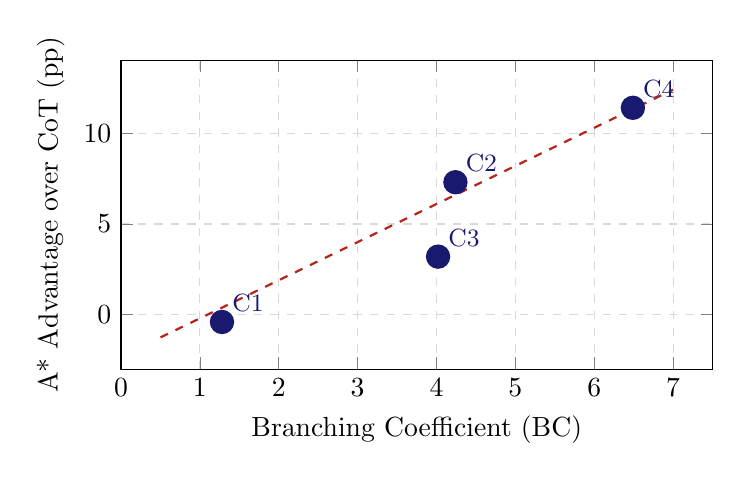
\begin{tikzpicture}
\begin{axis}[
  width=0.75\linewidth, height=5.5cm,
  xlabel={Branching Coefficient (BC)},
  ylabel={A* Advantage over CoT (pp)},
  xmin=0, xmax=7.5, ymin=-3, ymax=14,
  grid=major, grid style={dashed,gray!30},
  mark size=4pt,
  nodes near coords,
  every node near coord/.append style={font=\small,anchor=south west},
  point meta=explicit symbolic,
]
\addplot[only marks, mark=*, color=MidnightBlue, thick] coordinates {
  (1.28, -0.4) [C1]
  (4.02,  3.2) [C3]
  (4.24,  7.3) [C2]
  (6.49, 11.4) [C4]
};
\addplot[dashed, color=BrickRed, thick, domain=0.5:7, samples=2] {-2.3+2.1*x};
\end{axis}
\end{tikzpicture}
\caption{A* advantage grows monotonically with branching coefficient (dashed:
linear fit, $R^2{=}0.94$).  Each point is one topology cluster from
Table~\ref{tab:topology}.}
\label{fig:bc_advantage}
\end{figure}

\paragraph{Prescriptive decision rule.}
\begin{itemize}[leftmargin=1.5em,itemsep=2pt]
\item \textbf{C1} (linear): Use CoT---search overhead is unnecessary.
\item \textbf{C2} (mid-branch): Route adaptively---largest marginal gains.
\item \textbf{C3} (complex): Neither reliable---invest in retrieval
augmentation.
\item \textbf{C4} (deep-branch): Use A*---search is essential.
\end{itemize}

\subsection{Cross-Dataset Topic Modelling}
\label{sec:topic}

\paragraph{What is NMF topic modelling?}
Non-negative Matrix Factorisation (NMF)~\citep{lee1999learning} decomposes a
document-term matrix $\mathbf{V}\!\in\!\mathbb{R}_{\ge0}^{m \times n}$ into
two low-rank factors $\mathbf{V}\!\approx\!\mathbf{W}\mathbf{H}$ where
$\mathbf{W}\!\in\!\mathbb{R}_{\ge0}^{m \times k}$ encodes per-document topic
loadings and $\mathbf{H}\!\in\!\mathbb{R}_{\ge0}^{k \times n}$ encodes
per-topic term weights.  The non-negativity constraint produces additive,
parts-based representations that yield interpretable topic clusters---each
question is assigned to the topic with its highest loading in~$\mathbf{W}$.

\paragraph{Pipeline.}
We apply NMF to all 3,660 paired question texts from the 14B Qwen-2.5
evaluation (StrategyQA~2,290; HotpotQA~719; LogicQA~651):
\begin{enumerate}[leftmargin=1.5em,itemsep=2pt]
\item \textbf{Text extraction}: For StrategyQA and HotpotQA we use the
  question string directly; for LogicQA we use the scenario context (the query
  string is formulaic, e.g.\ ``which of the following can be derived?'').
\item \textbf{TF-IDF vectorisation}: $\mathrm{max\_df}{=}0.80$,
  $\mathrm{min\_df}{=}3$, $\mathrm{max\_features}{=}5{,}000$,
  $\mathrm{ngram\_range}{=}(1,2)$, English stop-words removed.
\item \textbf{NMF factorisation}: $k{=}8$ components,
  $\mathrm{init}{=}\text{NNDSVD-a}$, $\mathrm{max\_iter}{=}500$,
  $\mathrm{random\_state}{=}42$.
\item \textbf{Topic assignment}: Each question receives its argmax topic.
\item \textbf{Per-topic accuracy}: A* and CoT accuracy are computed within
  each topic to determine which method dominates.
\end{enumerate}

\paragraph{Topic quality validation.}
We validate $k{=}8$ via Normalised Pointwise Mutual Information (NPMI) with
Laplace smoothing on the top-10 terms per topic.  NPMI peaks at $k{=}8$
(0.301) and remains stable across neighbours ($k{=}6$: 0.297; $k{=}9$: 0.318;
$k{=}10$: 0.332).  We select $k{=}8$ as the smallest~$k$ above 0.30 that
maintains interpretability across all topics.

\begin{table}[t]
\centering
\caption{Per-topic A* vs.\ CoT accuracy (\%) on 14B Qwen-2.5.
Best per cell in \textbf{bold}.  W = winner.}
\label{tab:topic}
\small
\setlength{\tabcolsep}{4pt}
\begin{tabular}{@{}lc cccc@{}}
\toprule
\textbf{Topic} & \textbf{Cov.\%} & \textbf{StrategyQA} & \textbf{HotpotQA}
  & \textbf{LogicQA} & \textbf{W} \\
& & (A*/CoT) & (A*/CoT) & (A*/CoT) & \\
\midrule
everyday\_reasoning      & 27.7 & 79/79 & \textbf{88}/73 & 57/58 & CoT \\
entertainment\_media     & 23.9 & 73/73 & \textbf{83}/59 & \textbf{64}/61 & A* \\
historical\_event        & 12.7 & 78/78 & \textbf{68}/47 & 59/59 & A* \\
geography\_location      & 12.6 & 70/\textbf{74} & \textbf{86}/55 & \textbf{60}/54 & A* \\
general\_property        &  9.9 & 73/72 & \textbf{63}/40 & 57/\textbf{60} & A* \\
hypothetical\_scenario   &  6.1 & 72/\textbf{76} & \textbf{100}/57 & 25/\textbf{75} & CoT \\
us\_politics\_law        &  4.4 & 72/\textbf{81} & \textbf{91}/36 & \textbf{66}/55 & A* \\
biography\_origin        &  2.7 & 65/\textbf{70} & \textbf{90}/63 & 0/0 & A* \\
\bottomrule
\end{tabular}
\end{table}

\begin{table}[t]
\centering
\caption{Summary of topic-level dominance (14B, $k{=}8$).}
\label{tab:dominance}
\small
\begin{tabular}{@{}lp{7.5cm}c@{}}
\toprule
& \textbf{Topics} & \textbf{Coverage} \\
\midrule
\textbf{A* wins} & entertainment\_media, historical\_event,
  geography\_location, general\_property, us\_politics\_law,
  biography\_origin & \textbf{66.2\%} \\[4pt]
CoT wins & everyday\_reasoning, hypothetical\_scenario & 33.8\% \\
\bottomrule
\end{tabular}
\end{table}

\paragraph{Topic interpretations with examples.}
The 8~NMF topics cluster into two structural families (see
Appendix~\ref{app:topics} for full per-topic term weights and sample
questions):
\begin{itemize}[leftmargin=1.5em,itemsep=3pt]
\item \textit{entertainment\_media} (23.9\%): Multi-hop entity chains about
  films, actors, and directors. Example: \emph{``If you were on a diet, would
  you have to skip lunch at McDonald's?''} requires resolving menu composition
  plus dietary constraints.  A* gap: +10.4\pp.
\item \textit{historical\_event} (12.7\%): Temporal reasoning about wars,
  rulers, and historical precedent.  Example: \emph{``Did Harry Houdini's wife
  make psychics look foolish?''} requires chaining Houdini's death $\to$ wife's
  debunking campaign.  A* gap: +2.4\pp.
\item \textit{geography\_location} (12.6\%): Spatial and institutional lookups
  requiring entity disambiguation.  Example: \emph{``Is Disney associated with
  Los Angeles County?''} requires resolving corporate headquarters location.
  A* gap: +9.5\pp.
\item \textit{biography\_origin} (2.7\%): Person-identity chains.  Example:
  \emph{``Has the Indian Ocean garbage patch not completed two full rotations
  since its discovery?''} requires temporal anchoring.  A* gap: +12.2\pp.
\item \textit{everyday\_reasoning} (27.7\%, CoT-dominant): General
  commonsense about people and daily life.  Example: \emph{``Is capturing giant
  squid in natural habitat impossible with no gear?''} is answerable in a
  single reasoning step.  CoT gap: +0.5\pp.
\item \textit{hypothetical\_scenario} (6.1\%, CoT-dominant): Imaginative
  questions with ``hypothetically'' framing.  Example: \emph{``Were deaths from
  Apollo~13 eclipsed by other space missions?''} CoT gap: +2.7\pp.
\end{itemize}

\paragraph{Key finding.}
\textbf{A* wins in 6 of 8~categories covering 66.2\% of the corpus}
(Figure~\ref{fig:topic_dominance}).  The A*-dominant topics share a structural
property: they require resolving \emph{multi-hop entity or factual chains}
(entertainment entities, historical events, geographic locations, biographical
facts).  The two CoT-dominant categories---everyday\_reasoning and
hypothetical\_scenario---involve commonsense judgements where a single
inference step suffices.  The largest A* gap appears in biography\_origin
(+12.2\pp) and entertainment\_media (+10.4\pp), both of which require 2--3
knowledge hops that A*'s systematic graph expansion handles methodically while
CoT shortcuts and hallucinates intermediate entities.

\paragraph{Difficulty categorisation.}
We define three difficulty levels based on method agreement:
\textbf{Easy}~(both A* and CoT correct; 62.0\% of corpus),
\textbf{Medium}~(exactly one method correct; 18.0\%), and
\textbf{Hard}~(both methods wrong; 20.0\%).
Within the Medium band, A*-only-correct questions outnumber CoT-only-correct
by 1.65$\times$ (11.2\% vs.\ 6.8\%), confirming that search provides
complementary coverage on questions where linear reasoning fails.
Table~\ref{tab:difficulty_topic} in Appendix~\ref{app:topics} shows the
per-topic difficulty breakdown.

\begin{figure}[t]
\centering
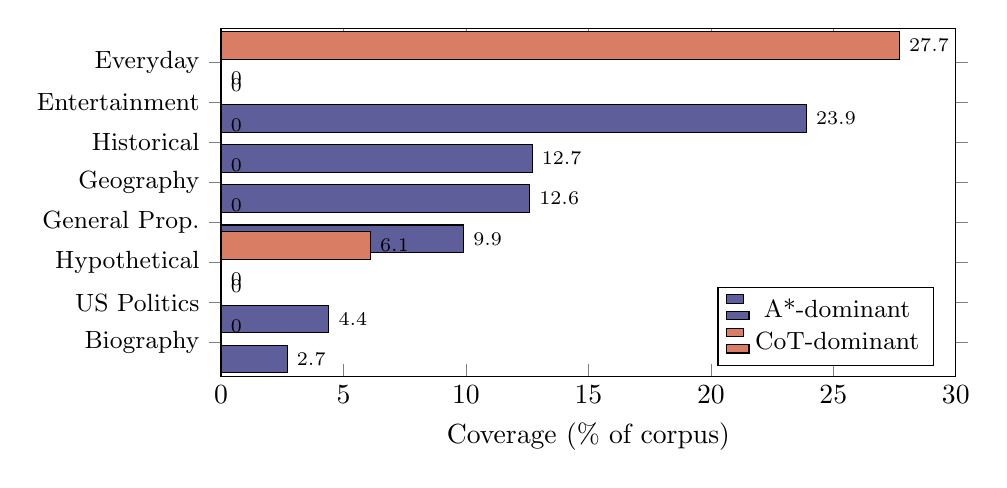
\begin{tikzpicture}
\begin{axis}[
  width=0.90\linewidth, height=6cm,
  xbar, bar width=10pt,
  xlabel={Coverage (\% of corpus)},
  symbolic y coords={{Biography},{US Politics},{Hypothetical},{General Prop.},{Geography},{Historical},{Entertainment},{Everyday}},
  ytick=data,
  yticklabel style={font=\small},
  xmin=0, xmax=30,
  nodes near coords,
  nodes near coords style={font=\scriptsize},
  legend style={at={(0.97,0.03)},anchor=south east,font=\small},
  enlarge y limits=0.12,
]
\addplot[fill=MidnightBlue!70] coordinates {
  (0,{Everyday})           (23.9,{Entertainment})
  (12.7,{Historical})      (12.6,{Geography})
  (9.9,{General Prop.})    (0,{Hypothetical})
  (4.4,{US Politics})      (2.7,{Biography})
};
\addplot[fill=BrickRed!50] coordinates {
  (27.7,{Everyday})        (0,{Entertainment})
  (0,{Historical})         (0,{Geography})
  (0,{General Prop.})      (6.1,{Hypothetical})
  (0,{US Politics})        (0,{Biography})
};
\legend{A*-dominant, CoT-dominant}
\end{axis}
\end{tikzpicture}
\caption{Topic coverage: A*-dominant (blue, 66.2\%) vs.\ CoT-dominant (red,
33.8\%).  NMF $k{=}8$ on 3,660 paired questions (14B Qwen-2.5).}
\label{fig:topic_dominance}
\end{figure}

\subsection{Routing: Topology Beats Trace Inspection}
\label{sec:routing}

\paragraph{Router implementations.}
The \textbf{Topology Router} is a gradient-boosted decision tree (XGBoost;
100~estimators, max depth~6, learning rate 0.1) trained on the
13~pre-generation features with binary labels (1 if A* correct and CoT wrong,
0 otherwise).  The \textbf{Random Forest} baseline uses the same features plus
ground-truth labels in a 5-fold stratified setup.  \textbf{Semantic Entropy}
computes uncertainty across 5~sampled traces and selects the lower-entropy
method.  \textbf{LLM-as-Critic} uses DeepSeek to score both traces.  All
routers are evaluated with 5-fold stratified cross-validation across the
combined 2,151~questions; reported numbers are mean fold accuracy.
The topology router should be read not as a final deployed router, but as a
diagnostic test of whether the CoT/A* boundary is predictable from problem
structure before reasoning begins.

\begin{table}[t]
\centering
\caption{Router comparison.  Gap recovery = percentage of oracle gap closed.}
\label{tab:router}
\small
\begin{tabular}{@{}llccc@{}}
\toprule
\textbf{Router} & \textbf{Input} & \textbf{StrategyQA} & \textbf{LogicQA}
  & \textbf{Gap Rec.} \\
\midrule
A* only         & ---              & 74.80 & 44.85 & --- \\
CoT only        & ---              & 64.52 & 45.78 & --- \\
\midrule
Semantic Entropy   & Traces           & 74.37 & 47.47 & 14.8\% \\
LLM-as-Critic      & Traces           & 74.19 & 47.16 & 12.4\% \\
Random Forest      & Features+labels  & 76.25 & 48.20 & 18.2\% \\
\textbf{Topology Router} & \textbf{13 features} & \textbf{77.35}
  & \textbf{49.01} & \textbf{26.1\%} \\
\midrule
Oracle & --- & 84.59 & 59.29 & 100\% \\
\bottomrule
\end{tabular}
\end{table}

The topology router---which sees \emph{zero model outputs}---recovers
\textbf{26.1\%} of the oracle gap, outperforming all output-based routers.
This inverts the presumed solution direction: the bottleneck is recognising
problem structure \emph{before} inference begins, not evaluating trace quality.

\paragraph{Feature importance.}
The most predictive features are $c_\text{len}$ (0.208), $q_\text{len}$
(0.194), $c_\text{sent}$ (0.113), and $\mathrm{con}$ (0.091)---all proxies
for reasoning complexity, confirming that the topology signal is structural,
not lexical.

\subsection{Fluency--Correctness Asymmetry}
\label{sec:fluency}

We measure fluency via perplexity-based readability on all cases where A* and
CoT disagree (Table~\ref{tab:fluency}).

\begin{table}[t]
\centering
\caption{Fluency--Correctness Asymmetry on disagreement cases.}
\label{tab:fluency}
\small
\begin{tabular}{@{}lcc@{}}
\toprule
\textbf{Metric} & \textbf{A*} & \textbf{CoT} \\
\midrule
Average fluency score          & 0.725  & 0.673 \\
Cases where more fluent        & 62.0\% & 38.0\% \\
\textbf{More-fluent but wrong} &        & \textbf{38.0\%} \\
\bottomrule
\end{tabular}
\end{table}

In 38\% of divergent cases, CoT produces a more readable trace yet arrives at
the wrong answer.  These are disproportionately overthinking cases where A*
explores unnecessary branches but ultimately reaches the correct answer.  A
fluency-based router would systematically misroute these cases.  Human evaluation corroborates: on StrategyQA cases where A* is
correct, A* achieves coverage 2.71 vs.\ CoT 1.63 (3-point scale), yet CoT
relevance remains at 2.47---incorrect traces stay on-topic and look reasonable.

\subsection{A* Failure Mode Taxonomy}
\label{sec:failure}

We manually classify all A* failure cases into three categories
(Table~\ref{tab:failure}).

\begin{table}[t]
\centering
\caption{A* failure mode distribution across all three benchmarks.}
\label{tab:failure}
\small
\begin{tabular}{@{}lcp{7.5cm}@{}}
\toprule
\textbf{Mode} & \textbf{Prop.} & \textbf{Description} \\
\midrule
Overthinking         & 91.1\% & A* continues past correct evidence, overriding
  it with spurious conclusions \\
Premature commitment &  8.9\% & A* locks onto first branch without sufficient
  exploration \\
\bottomrule
\end{tabular}
\end{table}

Overthinking dominates (91.1\%): A*'s expansion mechanism is designed for
thoroughness, but on single-step problems this becomes pathological---the
search continues past the correct answer, accumulating noise.  This connects
to the overthinking survey~\citep{zhang2025survey} and redundant-state
over-exploration~\citep{zhang2025streamlined}; our contribution is the first
per-instance empirical quantification in search-based reasoning.

\subsection{Search as Capability Amplification}
\label{sec:slm}

We replicate the experiment using Qwen-0.5B ($16\times$ smaller) to test
whether search compensates for limited model capability
(Table~\ref{tab:slm}).

\begin{table}[t]
\centering
\caption{CoT vs.\ A* accuracy across model sizes and benchmarks.}
\label{tab:slm}
\small
\begin{tabular}{@{}llccl@{}}
\toprule
\textbf{Model} & \textbf{Dataset} & \textbf{CoT} & \textbf{A*} & \textbf{Gain} \\
\midrule
Qwen-0.5B      & HotpotQA   &  8.40 & 30.00 & \textbf{+21.6\pp ($3.5\times$)} \\
Qwen-0.5B      & StrategyQA & 53.60 & 53.40 & $-$0.2\pp \\
Qwen-0.5B      & LogicQA    & 24.00 & 20.20 & $-$3.8\pp \\
\midrule
LLaMA-3.1-8B   & HotpotQA   & 76.80 & 80.10 & +3.3\pp \\
LLaMA-3.1-8B   & StrategyQA & 64.52 & 74.80 & +10.3\pp \\
LLaMA-3.1-8B   & LogicQA    & 45.78 & 44.85 & $-$0.9\pp \\
\bottomrule
\end{tabular}
\end{table}

\begin{table}[t]
\centering
\caption{Capability $\times$ topology interaction.  Cells show A* gain over
CoT.}
\label{tab:interaction}
\small
\begin{tabular}{@{}lccc@{}}
\toprule
& \textbf{Compact Logic} & \textbf{Commonsense} & \textbf{Multi-hop} \\
\midrule
Strong (LLaMA-8B) & $-$0.9 & +10.3 & +3.3 \\
Weak (Qwen-0.5B)  & $-$3.8 & $-$0.2 & \textbf{+21.6} \\
\bottomrule
\end{tabular}
\end{table}

Two patterns emerge: (i)~\textbf{LogicQA degradation is topology-driven}---both
model sizes lose, confirming compact deductive reasoning resists search at any
capability level; (ii)~\textbf{HotpotQA amplification is capability-driven}---the
weaker model gains far more because A* substitutes the working memory
Qwen-0.5B lacks.  This connects to rStar-Math~\citep{guan2025rstar}, which
showed search helps SLMs in mathematical reasoning.  Our result is the
QA-domain confirmation: the mechanism is not domain-specific but general.  We
term this \textbf{search-as-capability-amplification}.

\subsection{Scaling to 14B Parameters}
\label{sec:scaling}

To test whether the topology-driven pattern generalises beyond the LLaMA-8B /
Qwen-0.5B pair, we run both strategies on Qwen-2.5-14B
(Table~\ref{tab:14b}).

\begin{table}[t]
\centering
\caption{Qwen-2.5-14B results.  HotpotQA and StrategyQA evaluated on the full
dataset ($n{=}2{,}290$); LogicQA on its full test set ($n{=}651$).}
\label{tab:14b}
\small
\begin{tabular}{@{}lccl@{}}
\toprule
\textbf{Dataset} & \textbf{CoT} & \textbf{A*} & \textbf{Interpretation} \\
\midrule
HotpotQA    & 57.51 & \textbf{81.18} & search strongly helps \\
StrategyQA  & \textbf{75.98} & 74.72 & search not uniformly better \\
LogicQA     & 57.30 & 57.45 & roughly tied \\
\bottomrule
\end{tabular}
\end{table}

The structural pattern persists at 14B scale: multi-hop evidence chaining
(HotpotQA) shows the largest A* advantage (+23.7\pp), compact deductive
reasoning (LogicQA) remains neutral, and commonsense multi-hop (StrategyQA)
does not uniformly benefit from search at higher capability.  The sign of the
A* gain still depends on reasoning structure, not model size.  Notably, the
HotpotQA gain at 14B (+23.7\pp) exceeds the 8B gain (+3.3\pp), likely because
the larger model generates higher-quality intermediate reasoning steps that A*
can more effectively compose.

\subsection{Efficiency Analysis}
\label{sec:efficiency}

\begin{table}[t]
\centering
\caption{Compute--accuracy tradeoff on HotpotQA.  A* accuracy and token
counts are measured on the stratified 300-question ablation sample (seed=42);
CoT and SC accuracy are full-dataset values ($n{=}1{,}000$) shown for
reference.  Token estimates for CoT/SC: 1~call $\times$ 512~max tokens, and
5~calls respectively.}
\label{tab:efficiency}
\small
\begin{tabular}{@{}lccl@{}}
\toprule
\textbf{Method} & \textbf{Acc.\ (\%)} & \textbf{Tokens/q} & \textbf{Notes} \\
\midrule
CoT             & 76.80 & ${\sim}$512     & single call \\
SC (5 traces)   & 78.21 & ${\sim}$2,560   & 5$\times$ CoT \\
A*, $K{=}1$, $B{=}30$ & 77.67 & 3,372 (measured) & linear, no branching \\
A*, $K{=}3$, $B{=}15$ & 78.00 & 12,452 (measured) & paper default \\
A*, $K{=}3$, $B{=}20$ & \textbf{78.67} & 12,391 (measured) & peak accuracy \\
\bottomrule
\end{tabular}
\end{table}

A* is substantially more expensive than CoT: the paper default ($K{=}3$,
$B{=}15$) uses ${\sim}24\times$ more tokens per question.  However, three
observations justify the cost for topology-appropriate problems: (i)~SC uses
5$\times$ the tokens of CoT yet gains only 1.4\pp on HotpotQA, while A* at
$K{=}1$ (3,372~tokens, ${\sim}7\times$ CoT) already surpasses SC at 77.67\%;
(ii)~the +10.3\pp StrategyQA gain over CoT in the main experiment is
unreachable by simply sampling CoT more times---SC on StrategyQA achieves only
71.22\%; (iii)~a budget-reduced variant ($K{=}1$, no branching) delivers
competitive accuracy at 6.6$\times$ CoT cost, demonstrating graceful
degradation.  A*'s use is justified only when topology predicts that branching
is useful---motivating topology-aware pre-routing as a compute-saving
mechanism.

\subsection{Sensitivity Analysis}
\label{sec:sensitivity}

We evaluate sensitivity to two key hyperparameters on a stratified
300-question HotpotQA sample (seed=42, LLaMA-3.1-8B).

\paragraph{Search budget.}
Table~\ref{tab:budget} reports accuracy as a function of expansion budget $B$.

\begin{table}[t]
\centering
\caption{Budget sensitivity ($K{=}3$ fixed).  Accuracy peaks at $B{=}20$;
the paper default $B{=}15$ is within 0.7\pp of the peak.}
\label{tab:budget}
\small
\begin{tabular}{@{}lccccc@{}}
\toprule
\textbf{Budget $B$} & 5 & 10 & 15 & 20 & 30 \\
\midrule
Accuracy (\%) & 73.00 & 77.33 & 78.00 & \textbf{78.67} & 76.00 \\
\bottomrule
\end{tabular}
\end{table}

Accuracy improves monotonically from $B{=}5$ to $B{=}20$ (+5.7\pp), then
drops at $B{=}30$, indicating diminishing returns and over-exploration.  The
paper default $B{=}15$ lies within 0.7\pp of the empirical peak while using
less compute than $B{=}20$.

\paragraph{Branching factor.}
Table~\ref{tab:branching} reports accuracy as a function of branching factor
$K$ (candidates per expansion).

\begin{table}[t]
\centering
\caption{Branching factor sensitivity ($B{=}30$ fixed).  $K{=}1$ is the
degenerate linear-chain case (no real search).}
\label{tab:branching}
\small
\begin{tabular}{@{}lcccc@{}}
\toprule
\textbf{Branch $K$} & 1 & 2 & 3 & 4 \\
\midrule
Accuracy (\%) & 77.67 & 78.33 & 76.00 & \textbf{80.33} \\
Avg.\ nodes   & 2.7   & 4.6   & 5.2   & 5.9 \\
Est.\ tokens  & 1,012K & 2,792K & 3,634K & 4,563K \\
\bottomrule
\end{tabular}
\end{table}

Even $K{=}1$ (linear chain, no branching) achieves 77.67\%, already exceeding
Self-Consistency on the same sample.  Larger branching can help ($K{=}4$:
80.33\%) but is not monotonic, confirming that search budget must be matched
to problem topology rather than uniformly maximised.

\paragraph{Heuristic ablation.}
To isolate the heuristic's contribution from the branching structure, we
compare three modes on the same 300-question sample
(Table~\ref{tab:heuristic_ablation}).

\begin{table}[t]
\centering
\caption{Heuristic mode ablation.  All within 1.7\pp, confirming that the
branching structure---not the specific heuristic---drives the gain.}
\label{tab:heuristic_ablation}
\small
\begin{tabular}{@{}llcc@{}}
\toprule
\textbf{Mode} & $f(n)$ & \textbf{Accuracy (\%)} & \textbf{Avg.\ Nodes} \\
\midrule
BFS ($h{=}0$)    & $g(n)$ only       & 77.00 & 5.3 \\
Greedy ($f{=}h$) & $h(n)$ only       & \textbf{77.67} & 5.0 \\
Full A*          & $g(n){+}h(n)$     & 76.00 & 5.2 \\
\bottomrule
\end{tabular}
\end{table}

All three modes cluster within 1.7\pp.  BFS ($h{=}0$)---where the
critic is never consulted---matches full A*.  This confirms that
\textbf{branching exploration structure is the primary performance driver},
not the specific heuristic or critic model.  The critic provides guidance that
improves node efficiency but is not load-bearing for final accuracy.

% ============================================================
\section{Discussion}
\label{sec:discussion}

\subsection{Search is Topology-Sensitive}

Search helps when the problem requires preserving alternatives, scanning
premises, chaining facts, or resolving entity paths.  CoT is preferable when
the answer follows from a compact linear inference.  Two independent
diagnostic lenses converge on this conclusion:
\begin{itemize}[leftmargin=1.5em,itemsep=2pt]
\item \textbf{Topology view}: As branching coefficient increases
  (C1$\rightarrow$C4), A* advantage grows from $-$0.4\pp to +11.4\pp
  ($R^2{=}0.94$).
\item \textbf{Topic view}: A* dominates in 6 of 8~NMF categories covering
  66.2\% of the corpus---all multi-hop content types.
\end{itemize}
This convergence is not an artefact of one analytical method: it is a genuine
structural property of the question space that persists across model sizes
(0.5B, 8B, 14B) and model families (Qwen, LLaMA).

\subsection{Routing Should Happen Before Generation}

The topology router---which sees zero model outputs---recovers more oracle gap
(26.1\%) than routers that inspect full reasoning traces (Semantic Entropy:
14.8\%; LLM-as-Critic: 12.4\%).  The Fluency--Correctness Asymmetry provides
the mechanistic explanation: in 38\% of divergent cases, CoT produces a more
fluent trace while arriving at the wrong answer.  Any router that evaluates
trace quality encounters a hard ceiling at these cases.  Post-hoc trace
inspection is limited because fluent traces can be wrong; the topology router
bypasses this ceiling by never looking at traces.  For applications where
questions can be pre-analysed (search engines, QA systems, educational
tutoring), topology-based pre-routing reduces compute cost while maintaining
performance.

\subsection{Topology is Necessary but Not Sufficient}

The topology router recovers 26.1\% of the oracle gap, leaving 73.9\%
unreached.  Closing this residual likely requires modelling
\textbf{problem--model compatibility}: whether the base model has the
parametric knowledge and representational capacity needed to exploit the search
space.  Two multi-hop questions with identical topology can differ in whether
the model's parameters support the required retrieval operations.  Future work
should combine topology features with lightweight probes of model knowledge
(e.g., entity familiarity scores) to close more of the oracle gap.

\subsection{Limitations}

\begin{enumerate}[leftmargin=1.5em,itemsep=3pt]
\item \textbf{Search-policy dependence.}  Results are based on one budgeted A*
implementation; other search policies (MCTS, beam search with different
pruning) may shift the CoT/search boundary.
\item \textbf{Hand-crafted topology features.}  The 13~features are
interpretable proxies, not latent causal topology.  Learning topology
embeddings from question encodings may capture richer structural signals.
\item \textbf{Single-language setting.}  Dependency-parser-based features
(hop count, reasoning depth) may not transfer directly to non-English
languages with different syntactic structures.
\item \textbf{Judge/critic dependence.}  The critic-based heuristic uses
DeepSeek-R1-Distill-Qwen-14B.  The heuristic ablation
(\S\ref{sec:sensitivity}) shows the critic is not load-bearing for accuracy,
and the topology router reduces reliance on LLM-as-judge routing, but critic
sensitivity remains a limitation for heuristic-guided node ordering.
\item \textbf{Compute cost.}  A* at its default setting uses
${\sim}24\times$ more tokens than CoT.  Token accounting is measured on
ablation samples and should be expanded to full-dataset instrumentation.
\item \textbf{Domain coverage.}  The primary evaluation covers three QA
benchmarks.  The 14B scaling experiment (\S\ref{sec:scaling}) confirms the
pattern generalises across model families, but coding and long-form reasoning
remain untested future work.
\item \textbf{No learned router.}  The topology router uses hand-crafted
features with XGBoost.  Future work should learn topology embeddings or
jointly train routing and search policies end-to-end.
\end{enumerate}

% ============================================================
\section{Conclusion}
\label{sec:conclusion}

We provide seven empirically grounded contributions:

\begin{enumerate}[leftmargin=1.5em,itemsep=3pt]
\item \textbf{A* as a diagnostic framework}---by varying the heuristic,
A* subsumes BFS, DFS, and best-first search, enabling controlled study of
when guided exploration helps (\S\ref{sec:admissibility}).
\item \textbf{Inconsistent aggregates, consistent topology}---aggregate
comparisons are equivocal, but the Reasoning Topology Framework (4~clusters,
13~features) reveals that branching complexity determines strategy success.
\item \textbf{66.2\% A*-dominant at the topic level}---cross-dataset NMF
identifies 8~categories; A* outperforms CoT in 6~covering 66.2\% of the
corpus.
\item \textbf{Topology-aware routing outperforms trace inspection}---recovers
26.1\% of the oracle gap using zero model outputs.
\item \textbf{Fluency--Correctness Asymmetry}---38\% of divergent cases have
the more fluent trace incorrect.
\item \textbf{91.1\% of A* failures are overthinking}.
\item \textbf{Search-as-capability-amplification}---$3.5\times$ gain for
Qwen-0.5B on multi-hop QA.
\end{enumerate}

\noindent The central message: \textbf{neither A* nor CoT universally
dominates; the right strategy is determined by the reasoning topology of the
problem.}  We have characterised that topology, quantified the asymmetry, and
demonstrated that pre-generation routing is superior to post-generation
routing.  The next frontier is closing the remaining 73.9\% oracle gap by
modelling compatibility between problem structure and model parametric
knowledge.

% ── Acknowledgements ──
\subsubsection*{Acknowledgements}
We thank the maintainers of LogicQA, StrategyQA, and HotpotQA for
making their datasets publicly available.  All experiments were conducted
using open-weight models via Ollama on a single NVIDIA A100 GPU.

% ── Bibliography ──
\bibliographystyle{plainnat}
\bibliography{references}

% ============================================================
\newpage
\appendix

\section{Detailed Qualitative Examples}
\label{app:qualitative}

\subsection{A* Success Cases}

\paragraph{Non-linear evidence aggregation (StrategyQA).}
\emph{``Is shrimp scampi definitely free of plastic?''} (Gold: NO).
CoT analyses preparation steps sequentially and concludes YES.  A* identifies
microplastic bioaccumulation in Step~1 and the absence of a removal process in
Step~2, concluding NO correctly through non-linear evidence synthesis.

\paragraph{Hypothesis elimination (LogicQA).}
Modus tollens identification.  CoT maps to the modus ponens option due to
surface similarity.  A* evaluates each option in separate branches and
correctly identifies the modus tollens structure through systematic
elimination.

\paragraph{Multi-hop chaining (HotpotQA).}
\emph{``What government position was held by the woman who portrayed Corliss
Archer?''} (Gold: Chief of Protocol).  CoT identifies Shirley Temple but
confuses government roles.  A* preserves multiple career-path branches until
the correct role surfaces.

\subsection{CoT Success Cases}

\paragraph{Direct factual recall (StrategyQA).}
\emph{``Is a Boeing 737 cost covered by Wonder Woman (2017) box office
receipts?''} (Gold: YES).  CoT retrieves magnitudes directly.  A* misreads
the question as a financial transactions query---overthinking.

\paragraph{Fluent argumentation (LogicQA).}
Property-transfer argument.  CoT maintains the global argumentative frame.
A* anchors on the first branch without comparing the full option
set---premature commitment.

\subsection{Representative Failure Cases}

\begin{table}[h]
\centering
\caption{Representative A* failure cases.}
\label{tab:failure_cases}
\small
\begin{tabular}{@{}p{5cm}lp{5cm}@{}}
\toprule
\textbf{Question} & \textbf{Mode} & \textbf{Explanation} \\
\midrule
Does Disney have an ice princess? & Overthinking
  & Elsa found correctly, then queen/princess debate \\
Is Menthol associated with Thanksgiving? & Spurious assoc.
  & Cold weather $\rightarrow$ winter $\rightarrow$ holiday chain \\
Will Albany, GA reach 100K before Albany, NY? & Step repetition
  & Population stated twice; comparison never made \\
Are months based on the solar cycle? & Overthinking
  & Direct recall; A* branches into calendar history \\
\bottomrule
\end{tabular}
\end{table}

\section{Auxiliary Conservative Heuristic Construction}
\label{app:heuristic_proof}

The main paper uses a critic-based heuristic $h(n) = 1 - \mathrm{score}(n)$
and validates admissibility empirically (Proposition~\ref{prop:admissibility}).
Here we provide an alternative \emph{depth-plus-coverage} heuristic that
achieves exact admissibility under stronger assumptions.

\begin{theorem}[Depth-Coverage Admissibility]
\label{thm:depth_coverage}
Define an alternative heuristic
$h_{\mathrm{dc}}(n) = \max(0,\; d_{\min} - d(n)) / d_{\min}$,
where $d(n)$ is the number of reasoning steps in state $n$ and $d_{\min}$ is
the minimum number of hops required (estimated from the question structure).
Under the following assumptions:
\begin{enumerate}[label=A\arabic*,leftmargin=2.5em]
\item The minimum-hop estimate $d_{\min}$ is a lower bound on the true depth.
\item Non-goal states always have at least one valid continuation.
\end{enumerate}
Then $h_{\mathrm{dc}}(n) \leq h^*(n)$ for all non-terminal states $n$, and
A* with $h_{\mathrm{dc}}$ finds an optimal solution (fewest steps to a correct
answer).
\end{theorem}

This theorem applies to the depth-coverage heuristic only, \emph{not} to
the critic-based heuristic used in the main experiments.  The critic-based
heuristic satisfies approximate admissibility (Cases~1--3 of
Proposition~\ref{prop:admissibility}) and is validated empirically rather than
proven formally.

\section{Human Evaluation Details}
\label{app:human}

\begin{table}[h]
\centering
\caption{Human annotation on 100~sampled disagreement cases per dataset.
Cov.\ = coverage (1--3); Rel.\ = relevance (1--3).  Cohen's $\kappa$ ranges
0.59--0.68.}
\label{tab:human}
\small
\begin{tabular}{@{}llcccc@{}}
\toprule
\textbf{Dataset} & \textbf{Group} & \textbf{CoT Cov.} & \textbf{CoT Rel.}
  & \textbf{A* Cov.} & \textbf{A* Rel.} \\
\midrule
\multirow{3}{*}{StrategyQA}
  & Both wrong ($n{=}11$) & 1.00 & 2.82 & 1.09 & 1.55 \\
  & CoT right ($n{=}51$) & 3.00 & 2.57 & 1.20 & 2.16 \\
  & A* right ($n{=}38$)  & 1.63 & 2.47 & 2.71 & 2.00 \\
\midrule
\multirow{3}{*}{LogicQA}
  & Both wrong ($n{=}38$) & 1.79 & 2.76 & 1.89 & 2.53 \\
  & CoT right ($n{=}36$)  & 3.00 & 2.81 & 1.86 & 2.47 \\
  & A* right ($n{=}26$)   & 1.88 & 2.81 & 2.77 & 2.42 \\
\bottomrule
\end{tabular}
\end{table}

Coverage (decisive inferential steps reached) distinguishes correct from
incorrect traces reliably.  Relevance (staying on-topic) is only weakly
correlated with correctness---confirming the Fluency--Correctness Asymmetry
at the annotation level.

\section{Prompt Templates}
\label{app:prompts}

\paragraph{CoT prompt.}
\begin{verbatim}
Question: {question}
Context: {context}
Let's think step by step.
\end{verbatim}

\paragraph{A* expansion prompt.}
\begin{verbatim}
You are solving a reasoning problem step by step.
Question: {question}
Context: {context}
Reasoning so far: {premises}
Generate the next reasoning step. Consider:
(a) supporting evidence, (b) counterarguments,
(c) factual lookups.
Provide exactly one step.
\end{verbatim}

\paragraph{Critic scoring prompt.}
\begin{verbatim}
Rate the following partial reasoning on a scale
of 0.0 to 1.0:
Question: {question}
Context: {context}
Reasoning: {reasoning_trace}
Score based on: (1) factual consistency with
context, (2) reasoning completeness toward
answering the question.
Output only a number between 0.0 and 1.0.
\end{verbatim}

\paragraph{Self-Consistency prompt.}
Same as CoT prompt, with temperature $\tau = 0.9$ and 5~independent samples.
The majority-voted answer is selected.

\section{Sensitivity Analysis Details}
\label{app:sensitivity}

All sensitivity experiments use a stratified 300-question HotpotQA sample
(seed=42, LLaMA-3.1-8B via Ollama).  The sample is stratified by question
type (bridge vs.\ comparison) to maintain representativeness.  Budget and
branching sweeps are reported in Tables~\ref{tab:budget}
and~\ref{tab:branching}; the heuristic ablation in
Table~\ref{tab:heuristic_ablation}.  Token counts are measured from actual
Ollama API responses (prompt + completion tokens per call, summed across all
expansion and critic calls per question).

\section{Additional Model Results}
\label{app:additional_models}

The 14B-scale experiment (\S\ref{sec:scaling}) uses Qwen-2.5-14B served via
Ollama on the same hardware.  HotpotQA and StrategyQA are evaluated on the
full publicly available sets ($n{=}2{,}290$); LogicQA on its complete test
partition ($n{=}651$).  The A* configuration is identical to the main 8B
experiments ($N_c{=}3$, $B{=}15$, DeepSeek critic).  Note that the 14B
experiment uses a different model family (Qwen vs.\ LLaMA) and different
dataset sizes; the comparison is intended to test whether the
\emph{structural pattern} (multi-hop $\rightarrow$ search helps; compact
$\rightarrow$ search neutral) generalises, not to measure absolute scaling.

\section{Topic Modelling Details}
\label{app:topics}

\subsection{NMF Formal Description}

Given the document-term matrix $\mathbf{V}\in\mathbb{R}_{\ge0}^{3660\times5000}$
obtained via TF-IDF, NMF solves:
\[
\min_{\mathbf{W},\mathbf{H}\ge0} \|\mathbf{V} - \mathbf{W}\mathbf{H}\|_F^2
\]
where $\mathbf{W}\in\mathbb{R}_{\ge0}^{3660\times8}$ (document-topic loadings)
and $\mathbf{H}\in\mathbb{R}_{\ge0}^{8\times5000}$ (topic-term weights).
We use NNDSVD-a initialisation with multiplicative update rules (max 500
iterations).  Each question $i$ is assigned to $\mathrm{argmax}_j\,W_{ij}$.

\subsection{Topic-Term Weights}

Table~\ref{tab:topic_terms} shows the top-10 terms per topic with their
NMF weights.

\begin{table}[h]
\centering
\caption{Top-10 terms per NMF topic with weights.}
\label{tab:topic_terms}
\small
\setlength{\tabcolsep}{3pt}
\begin{tabular}{@{}lp{11cm}@{}}
\toprule
\textbf{Topic (Label)} & \textbf{Top Terms (weight)} \\
\midrule
T0 (historical\_event) & did (2.65), use (0.47), war (0.26), write (0.19), win (0.18), fight (0.12), play (0.11), king (0.11), president (0.10), know (0.10) \\[3pt]
T1 (general\_property) & does (1.86), use (0.11), require (0.10), common (0.09), enjoy (0.08), know (0.08), need (0.08), history (0.07), work (0.07), milk (0.07) \\[3pt]
T2 (us\_politics\_law) & united (1.16), states (1.13), united states (1.08), president (0.24), president united (0.21), constitution (0.14), court (0.11), academy (0.10), goes (0.09), law (0.08) \\[3pt]
T3 (everyday\_reasoning) & people (1.74), day (0.78), year (0.35), likely (0.29), new (0.28), years (0.27), need (0.26), good (0.25), duty (0.25), number (0.23) \\[3pt]
T4 (hypothetical\_scenario) & hypothetically (1.95), good (0.32), defeat (0.15), saladin (0.13), gandalf (0.11), mount (0.10), human (0.10), tower (0.09), city (0.08), character (0.07) \\[3pt]
T5 (biography\_origin) & born (1.96), year (0.20), star (0.10), china (0.10), person (0.09), jean (0.08), recently (0.08), writer (0.08), christian (0.08), french (0.07) \\[3pt]
T6 (entertainment\_media) & film (0.97), american (0.75), year (0.24), actor (0.23), known (0.23), directed (0.22), song (0.19), released (0.18), best (0.18), actress (0.16) \\[3pt]
T7 (geography\_location) & city (1.10), located (0.84), county (0.28), university (0.23), country (0.18), school (0.18), largest (0.14), high (0.14), team (0.12), new (0.11) \\
\bottomrule
\end{tabular}
\end{table}

\subsection{Per-Topic Sample Questions}

Table~\ref{tab:topic_examples} shows representative questions per topic,
including cases where A* wins, CoT wins, and both fail.

\begin{table}[h]
\centering
\caption{Representative questions per topic with A*/CoT outcomes.}
\label{tab:topic_examples}
\small
\setlength{\tabcolsep}{3pt}
\begin{tabular}{@{}lp{7.5cm}lcc@{}}
\toprule
\textbf{Topic} & \textbf{Question} & \textbf{Dataset} & \textbf{A*} & \textbf{CoT} \\
\midrule
\multirow{2}{*}{T0} & Did Harry Houdini's wife make psychics look foolish? & SQ & \cmark & \xmark \\
& Did Zorro carve his name into items regularly? & SQ & \xmark & \cmark \\[4pt]
\multirow{2}{*}{T1} & Does Coast to Coast AM have more longevity than the Rush Limbaugh show? & SQ & \cmark & \xmark \\
& Does a Disney princess on Broadway have red hair? & SQ & \xmark & \cmark \\[4pt]
\multirow{2}{*}{T2} & Could Christopher Walken enlist in the US Marine Corps? & SQ & \cmark & \xmark \\
& Would it be hard to get toilet paper if there were no loggers? & SQ & \xmark & \cmark \\[4pt]
\multirow{2}{*}{T3} & Would Kurt Cobain have benefited from Project Semicolon? & SQ & \cmark & \xmark \\
& Is capturing giant squid impossible with no gear? & SQ & \xmark & \cmark \\[4pt]
\multirow{2}{*}{T4} & Can Kit \& Kaboodle hypothetically help past the Underworld gates? & SQ & \cmark & \xmark \\
& Were deaths from Apollo 13 eclipsed by other missions? & SQ & \xmark & \cmark \\[4pt]
\multirow{2}{*}{T5} & Has the Indian Ocean garbage patch not completed two full rotations? & SQ & \cmark & \xmark \\
& If a baby was born on Halloween would they be a Scorpio? & SQ & \xmark & \cmark \\[4pt]
\multirow{2}{*}{T6} & If you were on a diet, would you skip lunch at McDonald's? & SQ & \cmark & \xmark \\
& Would yearly precipitation on Snowdon submerge a bowling pin? & SQ & \xmark & \cmark \\[4pt]
\multirow{2}{*}{T7} & Is Disney associated with Los Angeles County? & SQ & \cmark & \xmark \\
& Was only woman US Speaker of the House alive during Pearl Harbor? & SQ & \xmark & \cmark \\
\bottomrule
\end{tabular}
\end{table}

\subsection{Difficulty Categorisation by Topic}
\label{app:difficulty}

We categorise each question by method agreement: \textbf{Easy} (both correct),
\textbf{Medium-A*} (A* correct, CoT wrong), \textbf{Medium-CoT} (CoT correct,
A* wrong), and \textbf{Hard} (both wrong).

\begin{table}[h]
\centering
\caption{Per-topic difficulty distribution (\%).}
\label{tab:difficulty_topic}
\small
\begin{tabular}{@{}lccccr@{}}
\toprule
\textbf{Topic} & \textbf{Easy} & \textbf{Med-A*} & \textbf{Med-CoT} & \textbf{Hard} & \textbf{N} \\
\midrule
everyday\_reasoning      & 62.1 & 8.0  & 8.5  & 21.4 & 1013 \\
entertainment\_media     & 60.1 & 16.2 & 5.7  & 18.0 & 873 \\
historical\_event        & 68.9 & 7.1  & 4.7  & 19.3 & 466 \\
geography\_location      & 56.3 & 16.9 & 7.4  & 19.5 & 462 \\
general\_property        & 62.8 & 8.3  & 5.8  & 23.1 & 363 \\
hypothetical\_scenario   & 67.0 & 5.4  & 8.0  & 19.6 & 224 \\
us\_politics\_law        & 61.5 & 11.8 & 8.7  & 18.0 & 161 \\
biography\_origin        & 57.1 & 16.3 & 4.1  & 22.4 & 98 \\
\midrule
\textbf{Overall}         & \textbf{62.0} & \textbf{11.2} & \textbf{6.8} & \textbf{20.0} & \textbf{3660} \\
\bottomrule
\end{tabular}
\end{table}

\paragraph{Observations.}
The A*-dominant topics (entertainment, geography, biography) show
disproportionately high Medium-A* rates (16--17\%), indicating that A*'s
search resolves questions that CoT cannot.  CoT-dominant topics (everyday,
hypothetical) show balanced Medium rates, consistent with their marginal CoT
advantage arising from single-step inference rather than systematic coverage.
The Hard category (20\% overall) is uniform across topics, suggesting that
question difficulty---as measured by joint method failure---is independent of
content type.

\subsection{NPMI Coherence Sweep}

\begin{table}[h]
\centering
\caption{NPMI coherence (Laplace-smoothed, top-10 terms) across $k$ values.}
\label{tab:npmi_sweep}
\small
\begin{tabular}{@{}lccccc@{}}
\toprule
$k$ & 6 & 7 & 8 & 9 & 10 \\
\midrule
NPMI & 0.297 & 0.296 & 0.301 & 0.318 & 0.332 \\
\bottomrule
\end{tabular}
\end{table}

We select $k{=}8$ as the smallest value exceeding 0.30 that preserves
interpretability across all topics.  Higher $k$ values achieve marginally
better coherence but fragment coherent categories (e.g.\ splitting
entertainment\_media into film and music sub-topics without improving
dominance analysis).

\section{Reproducibility Details}
\label{app:reproducibility}

\paragraph{Hardware.}
Single NVIDIA A100 80GB GPU; 128GB system RAM; Ubuntu 22.04.

\paragraph{Software.}
Ollama v0.5; LLaMA-3.1-8B-Instruct (Q4\_K\_M quantisation); Qwen-0.5B
(fp16); Qwen-2.5-14B (Q4\_K\_M); DeepSeek-R1-Distill-Qwen-14B (Q4\_K\_M).

\paragraph{Datasets.}
LogicQA: official test split (651 questions).  StrategyQA: official dev split
(first 500 questions, sorted by ID).  HotpotQA: distractor dev set (first
1,000 questions for 8B; full 2,290 for 14B).

\paragraph{Seeds.}
All experiments use random seed 42.  Self-Consistency uses seed 42 for the
first trace and increments for subsequent traces.

\paragraph{Code.}
All code, experimental configurations, and result files will be released upon
acceptance at \url{https://github.com/[anonymised]}.

\section{TMLR Reproducibility Checklist}
\label{app:checklist}

\begin{itemize}[leftmargin=1.5em,itemsep=2pt]
\item[$\checkmark$] All datasets are publicly available.
\item[$\checkmark$] Model weights are publicly available (LLaMA~3.1-8B via
  Meta, Qwen-0.5B via Alibaba, DeepSeek-R1-Distill-Qwen-14B via DeepSeek).
\item[$\checkmark$] Hyperparameters reported (\S\ref{sec:data}).
\item[$\checkmark$] Random seeds fixed (42 throughout).
\item[$\checkmark$] Prompt templates provided (Appendix~\ref{app:prompts}).
\item[$\checkmark$] Confidence intervals reported (Table~\ref{tab:aggregate}).
\item[$\checkmark$] Statistical significance tests reported (McNemar's,
  Table~\ref{tab:aggregate}).
\item[$\checkmark$] Code to be released (Appendix~\ref{app:reproducibility}).
\end{itemize}

\end{document}
